\uuid{U5NL}
\exo7id{7123}
\titre{exo7 7123}
\auteur{megy}
\organisation{exo7}
\datecreate{2017-02-08}
\isIndication{false}
\isCorrection{true}
\chapitre{Géométrie affine euclidienne}
\sousChapitre{Géométrie affine euclidienne du plan}
\module{Géométrie}
\niveau{L2}
\difficulte{}

\contenu{
\texte{
% application directe
Soient $\mathcal C_1$ et $\mathcal C_2$ deux cercles sécants en $A$ et $B$, et $\mathcal D_A$ (respectivement $\mathcal D_B$) une droite passant par $A$  (resp. $B$). On note $C$ et $E$ (resp. $D$ et $F$) l'intersection de $\mathcal D_A$ (resp. $\mathcal D_B$) avec 
 les deux cercles. Montrer que $(CD) // (EF)$.
}
\reponse{
Traçons une figure. \emph{On marque dès à présent quelques égalités d'angles obtenues par le théorème de l'angle inscrit:}

\begin{center}
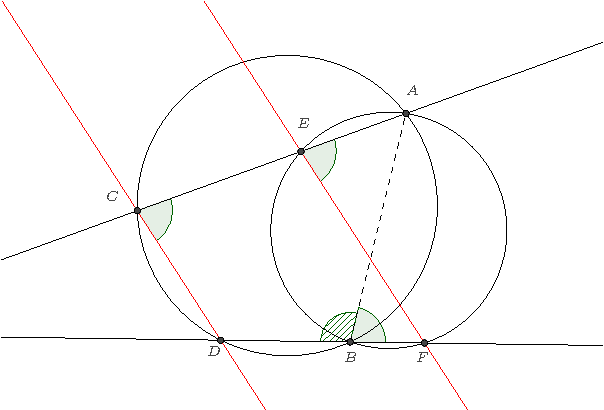
\includegraphics{../images/pdf/U5NL-1.pdf}
\end{center}

\emph{Les égalités d'angles repérées sur la figure permettent de voir la solution, au moins dans la configuration particulière dessinée. On voit en effet que les angles $\widehat{ECD}$ et $\widehat{AEF}$ sont égaux. Attention toutefois, les angles géométriques sont trompeurs et les égalités que l'on voit sur une figure peuvent dépendre de la façon de tracer la figure. Sur la figure ci-dessous par exemple, les angles en question ne sont pas égaux mais supplémentaires.}

\begin{center}
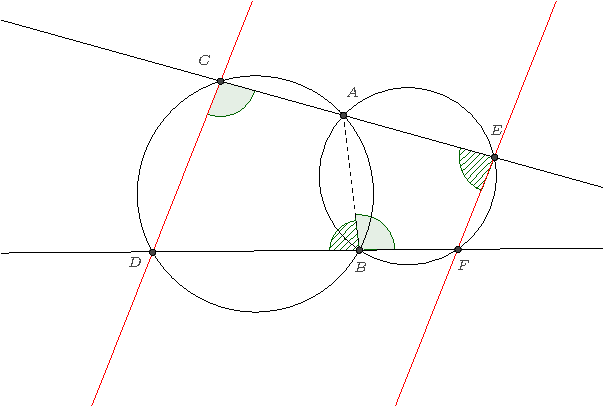
\includegraphics{../images/pdf/U5NL-2.pdf}
\end{center}


\emph{Il ne reste plus qu'à rédiger rigoureusement la solution  avec des angles de droites, en s'appuyant sur l'intuition donnée par la figure.}

Pour montrer que $(CD)$ et $(EF)$ sont parallèles, il suffit par exemple de montrer qu'elles forment le même angle avec la droite $(CA)$. Or on a la suite d'égalités d'angles de droites :

\begin{align*}
(CD,CA) &= (BD,BA) \text{ car $CDAB$ est inscriptible}\\
&= (BF,BA) \text{ car $(BD)=(BF)$}\\
&=(EF,EA) \text{ car $BFAE$ est inscriptible}\\
&=(EF,CA)  \text{ car $(EA)=(CA)$.}
\end{align*}
}
}
